% THESIS CHAPTER

\chapter{System description}
\label{chap:third}
\ifpdf
    \graphicspath{{Chapter3/Figures/PNG/}{Chapter3/Figures/PDF/}{Chapter3/Figures/}}
\else
    \graphicspath{{Chapter3/Figures/EPS/}{Chapter3/Figures/}}
\fi

% short summary of the chapter
\section*{Summary}

This chapter introduces the reader the current laboratory setup. The first section illustrates which kind of tools are used as well as the specifications of each component. The second section instead will present the integration both at hardware and software levels of each part of the system. 

\section{The setup}
\label{sec:setup}
This section introduces and explains the tools, both hardware and software, that are used in the experiments. 

We can identify five distinct parts:
\begin{itemize}
\item  IRIS quadcopter from 3D robotics
\item  Motion Capture system from Optitrack
\item  Linux workstation
\item  Windows machine
\item  Flight arena
\end{itemize}
While IRIS, the mocap system and the flight arena deserve three separate sections, the role of two machines is described in the integration part (see Section \ref{sec:integration}).

\subsection{IRIS Quadcopter}

The IRIS quadcopter is flying robot manufactured by 3D Robotics and commercially available as a kit or ready-to-fly. IRIS flight control system employs by default the open source software ArduPilot running on a Pixhawk autopilot board (based on the PX4 hardware developed by ETH).

\begin{figure}[h]
\centering
 \noindent
 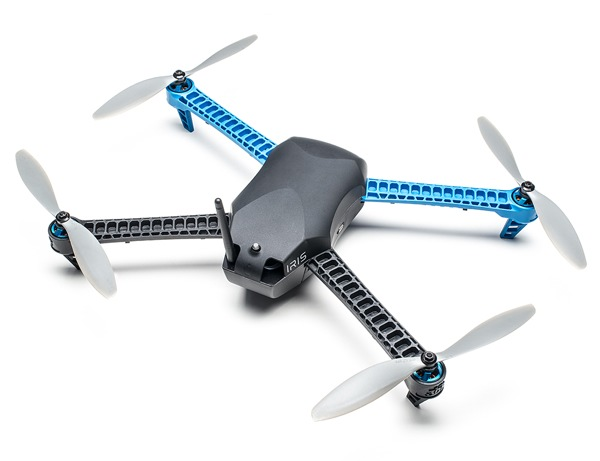
\includegraphics[width=0.8\textwidth]{iris.jpg}
 \caption{The IRIS quad copter}
 \label{figure:iris}
\end{figure}
\noindent
The main distinct components of the IRIS quadcopter are the airframe (central body, arms, motors and legs), four 850 kV DC brushless motors controlled in open-loop through PWM, one 11.1 V LiPo battery and control electronics.\\ 
The use is mainly commercial, it is optimized for aerial shooting and provides a lot of features the user can play with. IRIS can be easily setup to follow any GPS-enabled Android device with OTG compatibility, this technology controls also the gimbal to keep the camera centered on the target capturing videos and actually becoming a free hand camera. Using the free DroidPlanner app, the user can plan flights by simply drawing a flight plan on any Android tablet or phone. This allows for hands free flight control with virtually unlimited waypoints even keeping IRIS pointing to the same location via a Region of Interest (ROI) waypoint throughout the entire flight \cite{IRIS}.


\begin{figure}[h]
 \centering
 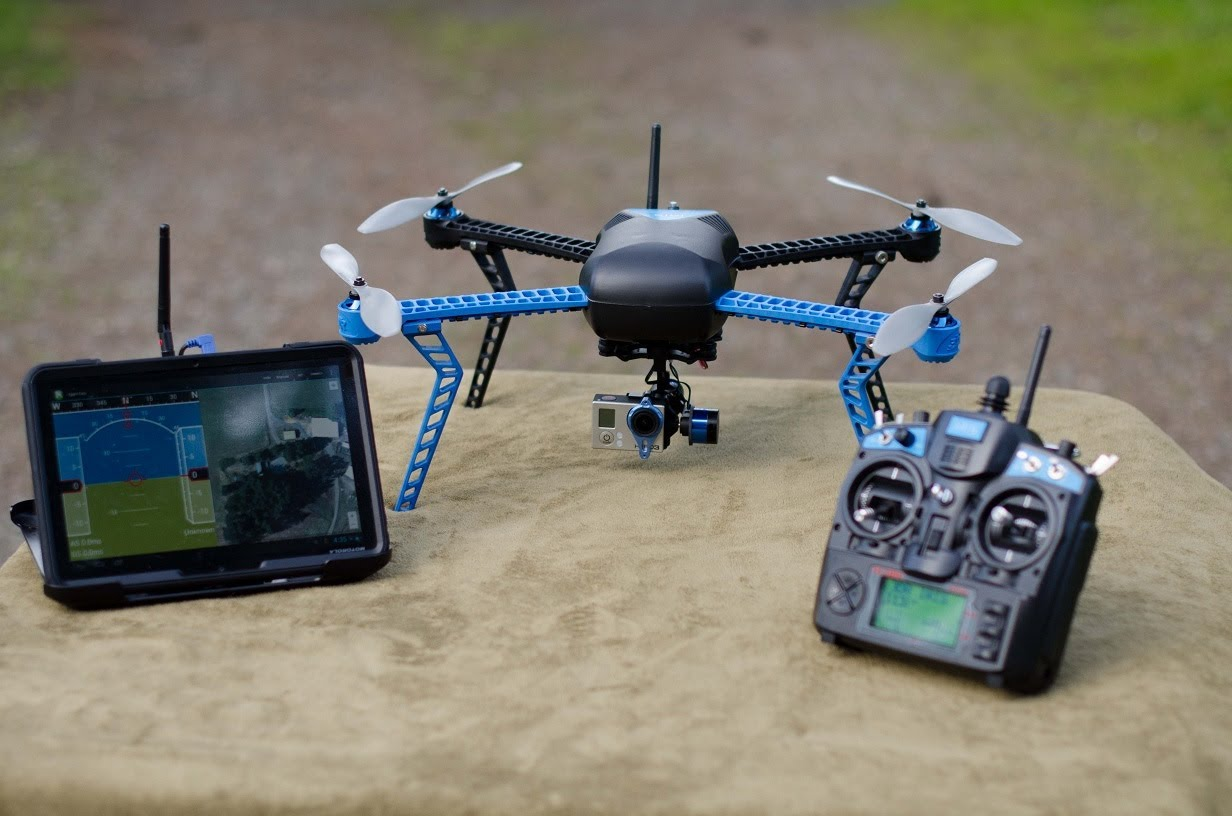
\includegraphics[width=0.6\textwidth]{iris_planner.jpg}
 \caption[IRIS and control devices]{IRIS and control devices.}
 \label{figure:iris_planner}
\end{figure}
This device is designed to fly outdoor, nevertheless it is possible with some software tuning to use the IRIS in indoor scenarios. The component which makes this possible is the actual brain of the robot: the PixHawk board with PX4 software. 

\subsubsection{PixHawk board}
\label{sec:pixboard}
PIXHAWK (figure \ref{figure:pixhawk}) is a high-performance autopilot-on-module suitable for fixed wing, multi rotors, helicopters, cars, boats and any other robotic platform that can move. It is targeted towards high-end research, amateur and industry needs and includes all hardware required for remote control \cite{PiXH}, stabilization and navigation functions namely:

\begin{itemize}
\item an embedded processor (32bit STM32F427 Cortex M4 core with FPU)
\item a fail-safe processor (32 bit STM32F103 failsafe co-processor)
\item a set of motion sensors, including an Inertial Measurement Unit sensing accelerations and angular speeds of the aircraft, a barometer to compute relative altitude and vertical speed from changes in static air pressure, a magnetometer for compass and a GPS receiver.

\item ESCs (Electronic Speed Controllers) that handle low-level motors control loops to maintain required thrust through open-loop PWM control.

\item RC Radio to receive direct pilot commands from an RC hand-held controller (2.4 GHz radio link).
\item telemetry module, a digital radio transceiver (433 MHz) receiving commands from the ground control station and sending telemetry data back to the ground via the \textit{MAVLink} protocol.
\end{itemize}

\begin{figure}[h]
 \centering
 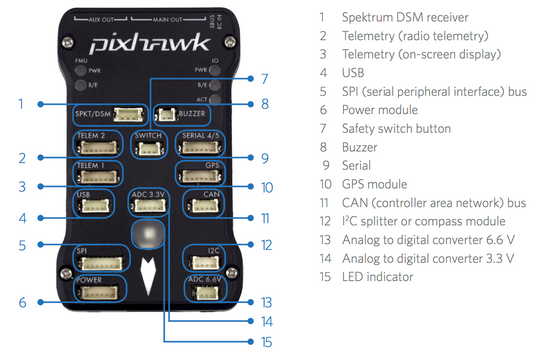
\includegraphics[width=0.8\textwidth]{pixhawk.PNG}
 \caption[Pixhawk board]{Pixhawk board and its connections.}
 \label{figure:pixhawk}
\end{figure}


It supports redundant technology both for power and processor, it is equipped with various interfaces such as CAN, SPI, I2C, UART and supports a micro USB for on board real time logging.

\subsubsection{PX4 Autopilot}
\label{sec:px4autop}
PX4 \cite{PX4} is the software stack running on the autopilot board, it was a master thesis project at ETH pursued by Lorenz Meier and it became a big open source project on github \cite{PX4Git} with contributors from all over the world. It works on NuttX \cite{Nutty} which is an open source real time OS and it uses uOrb (micro orb) as middleware. Different modules runs in parallel and they can be grouped in different sets:

\begin{itemize}

\item PX4 Flight Stack (estimation and control, cross-platform), the core modules dealing in this thesis
\item PX4 Middleware (ORB, NuttX )
\item PX4 ESC Firmware (for motor controllers)
\item PX4 Bootloader (for STM32 boards)
\item Operating System (NuttX or Linux/Mac OS)

\end{itemize}

\subsubsection{MAVLink Protocol}
\label{sec:mavlink}
MAVLink is a very lightweight, header-only message for micro air vehicles created and released under LGPL licence by Lorenz Meier in 2009.
It can pack, with very little overhead, C structs over serial channels with high effiency and send these packets to the ground control station (Fig. \ref{figure:controlstation}). It is extensively tested on the PX4, PIXHAWK, APM and Parrot AR.Drone platforms. It has the possibility to be used with at maximum of 255 vehicles on the same control station, it runs on multiple microcontrollers and OS such as  ARM7, ATMega, dsPic, STM32 or Windows, Linux, MacOS and iOS with only 8 byte of overhead. The intense testing of this protocol made it the most used communication protocol in aerial robotics due to his effectiveness. Mavlink is used to send message over radio link in this project.
\begin{figure}[H]
 \centering
 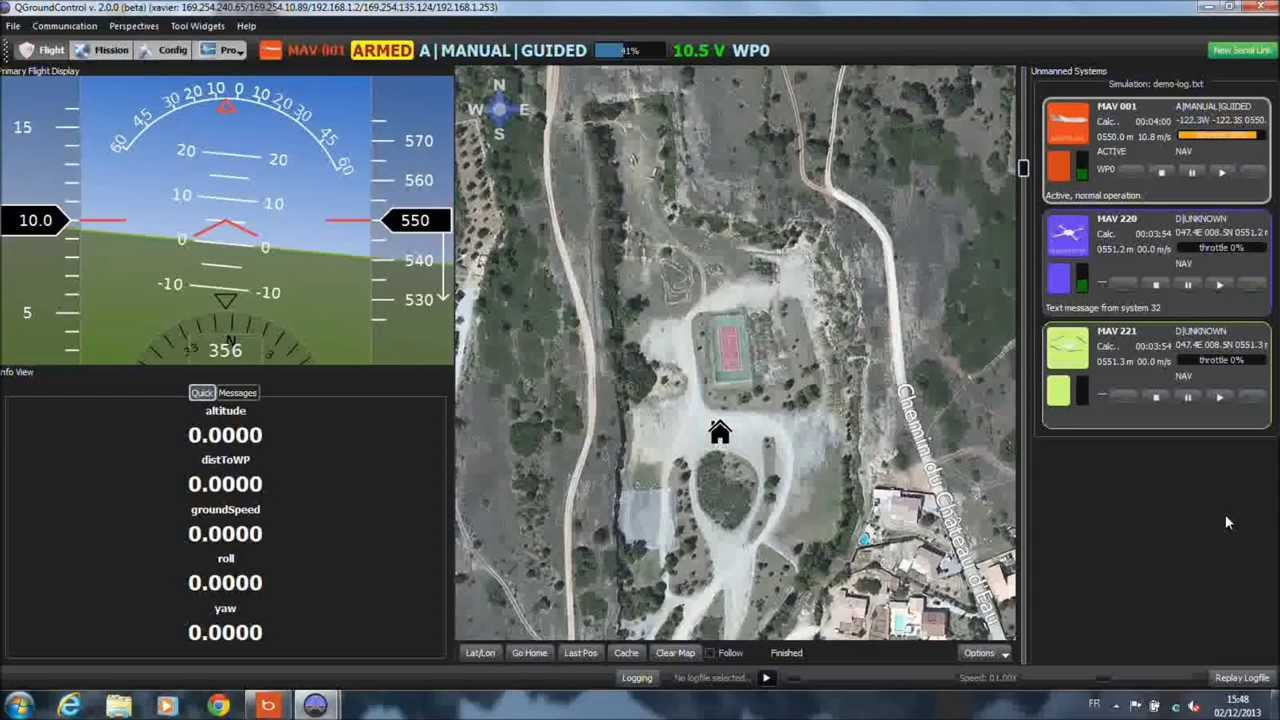
\includegraphics[width=0.9\textwidth]{groundcontrol.jpg}
 \caption[Ground Control Station]{Ground Control Station used to visualize robot parameters, plan missions or calibrate sensors.}
 \label{figure:controlstation}
\end{figure}


\paragraph{Supported data types}
MavLink supports fixed-size integer data types, IEEE 754 single precision floating point numbers, arrays of these data types and the special MavLink version field, which is added automatically by the protocol. Table \ref{tab:mavlink} contains a list of every data type that can be transported by MavLink packets \cite{MAVLink}.\par
\begin{table}
\centering
\begin{tabular}{c | p{6cm}}
\multicolumn{2}{c}{\large Mavlink supported Data types}\\
\hline
 \texttt{uint8\_t} &  Unsigned 8 bit\\
 \texttt{int8\_t} & Signed 8 bit\\
 \texttt{uint16\_t} &  Unsigned 16 bit\\
 \texttt{int16\_t} & Signed 16 bit\\
 \texttt{uint32\_t} & Unsigned 32 bit\\
 \texttt{int32\_t} & Signed 32 bit \\
 \texttt{uint64\_t} & Unsigned 64 bit \\
 \texttt{uint64\_t} &  Signed 64 bit \\
 \hline
 char & Characters or strings\\
 float & IEEE 754 single precision floating point number\\
 double & IEEE 754 double precision floating point number\\
 \hline
 \texttt{uint8\_t\_mavlink\_version}] & Unsigned 8 bit field automatically filled on sending with the current MAVLink version - it cannot be written, just read from the packet like a normal \texttt{uint8\_t} field
\end{tabular}
\caption[Mavlink types]{Mavlink supported data types.}
\label{tab:mavlink}
\end{table}
This protocol was designed towards two properties: transmission speed and safety. It allows to check the message content, it also allows to detect lost messages but still only needs six bytes overhead for each packet as illustrated in figure \ref{figure:MAV_anatomy}. Regarding the packets size we have that:

\begin{itemize}
\item The minimum packet length is 8 bytes for acknowledge packets without payload
\item The maximum packet length is 263 bytes for full payload
\end{itemize}

\begin{figure}[h]
 \centering
 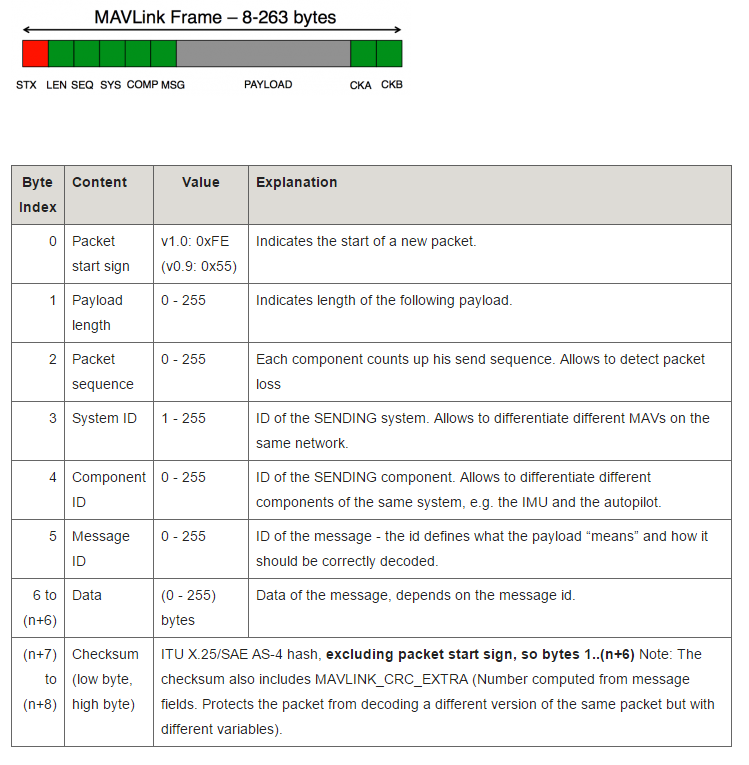
\includegraphics[width=0.8\textwidth]{MAVPack.PNG}
 \caption[MAVLink package anatomy]{MAVLink package anatomy.}
 \label{figure:MAV_anatomy}
\end{figure}

\newpage
\subsection{Motion capture system}
\label{sec:mocap}
The localization of the robot in 3D space relies on the OptiTrack FLEX 13 motion capture system, composed by 8 infrared cameras (Fig. \ref{figure:flex13}) mounted on the roof of the laboratory in a squared fashion around the flight perimeter. It is the mid level product in OptitTrack catalog (1000 dollars per camera \cite{OptiT}) capable of tracking multiple objects in a medium volume space of about $4 \times 4 \times 4$ meters.

\begin{figure}[h]
 \centering
 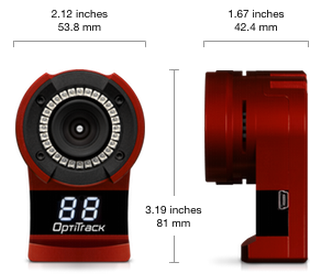
\includegraphics[width=0.6\textwidth]{flex13.PNG}
 \caption[Flex 13 Cameras]{Flex 13 camera and dimensions.}
 \label{figure:flex13}
\end{figure}


\subsubsection{Image sensor specifications and performances}
\begin{itemize}
\item Latency: 8.3 ms.
\item Frame Rate: 30-120 FPS (adjustable).
\item Imager Resolution: 1280 X 1024 (1.3 Megapixels).
\end{itemize}
\noindent
This camera features a status LED and a 2 digits numerical screen for diagnostics, mounting supports, an image sensor and a lens. A 28 LED ring around the lens ensures the required IR (Infra Red) illumination both in stroboscopic and continuous modes.

Object are defined by attaching to them at least 3 \textbf {passive infrared markers} (Figure \ref{figure:marker}) able to reflect infrared light, solving rigid bodies and ensure tracking. The number of markers that the OptiTrack is capable of tracking depends on the size of the markers and the distance they are from the camera. This number may change from model to model but is about 100 in our case, more than enough for this project.\par The 3D location of markers can be resolved with millimeter accuracy and resolution depending on capture volume size and camera configuration. Increasing the number of cameras can help improve the tracking performance if needed and in this case 0.3 mm of error for each marker is achieved. \\* 

\begin{figure}[h]
\centering
 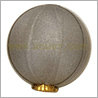
\includegraphics[width=0.2\textwidth]{marker.jpg}
 \caption[Passive IR marker]{Passive IR marker able to reflect IR radiation}
 \label{figure:marker}
\end{figure}


\subsubsection{Software, cameras layout and requirements} 

The system uses the proprietary software Motive \cite{OptiT}, an Optical motion capture software which incorporates many features such as rigid body solving and marker tracking. Motive is able to manage every camera parameter such as exposure, brightness and gain as well as the overall calibration.
Two USB hubs divide the eight cameras in two groups collecting four USB cables each coming from each sensor. Both hubs are connected through USB cables to the Windows machine where Motive is installed, moreover a sync cable responsible for the synchronization runs from one hub to the other.
Figure \ref{figure:hub} explains the connections of a single hub.
\\*

\begin{figure}[H]
\centering
 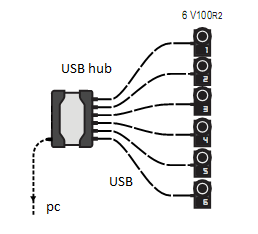
\includegraphics[width=0.5\textwidth]{HUB.png}
 \caption[Single hub connection]{Example of a single hub attached to 6 cameras, sync cable between the two hubs is not shown.}
 \label{figure:hub}
\end{figure}

\begin{figure}[h]
\centering
 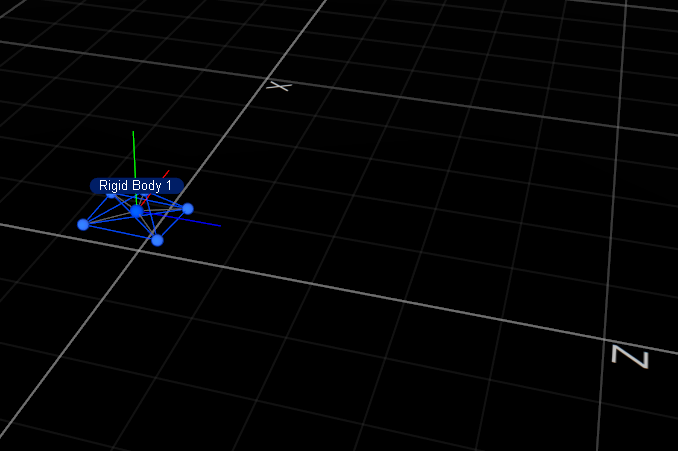
\includegraphics[width=0.7\textwidth]{motiv_iris.PNG}
 \caption[IRIS Rigid body]{IRIS Rigid body created with Motive software.}
 \label{figure:motivescreen}
\end{figure}
\noindent
The reader must note that in order to have a good tracking performance, the setup needs to assure some properties during the experiments:

\begin{itemize}
\item At least 3 markers must be present on the object.
\item The distance between each marker must be constant during the tracking period (Rigid body assumption).
\item Cameras must see at least 3 markers of the tracked rigid body.
\item Occlusions are not taken into account by Motive \cite{OptiT}.
\item Rigid bodies with symmetric shapes induce big uncertainties in attitude estimation.
\end{itemize}
I solved this problems mainly in two ways. Pointing each camera to the center of the flight space approximately at 0.5 meters from the ground gives the best coverage and few unseen areas at the margins.

Regarding the robot, with 5 markers placed in a 3D asymmetrical configuration  on the body frame as in figure \ref{figure:markedIRIS},is assured that at least 3 markers are always visible and there are no singularity regarding attitude.

\begin{figure}[h]
\centering
 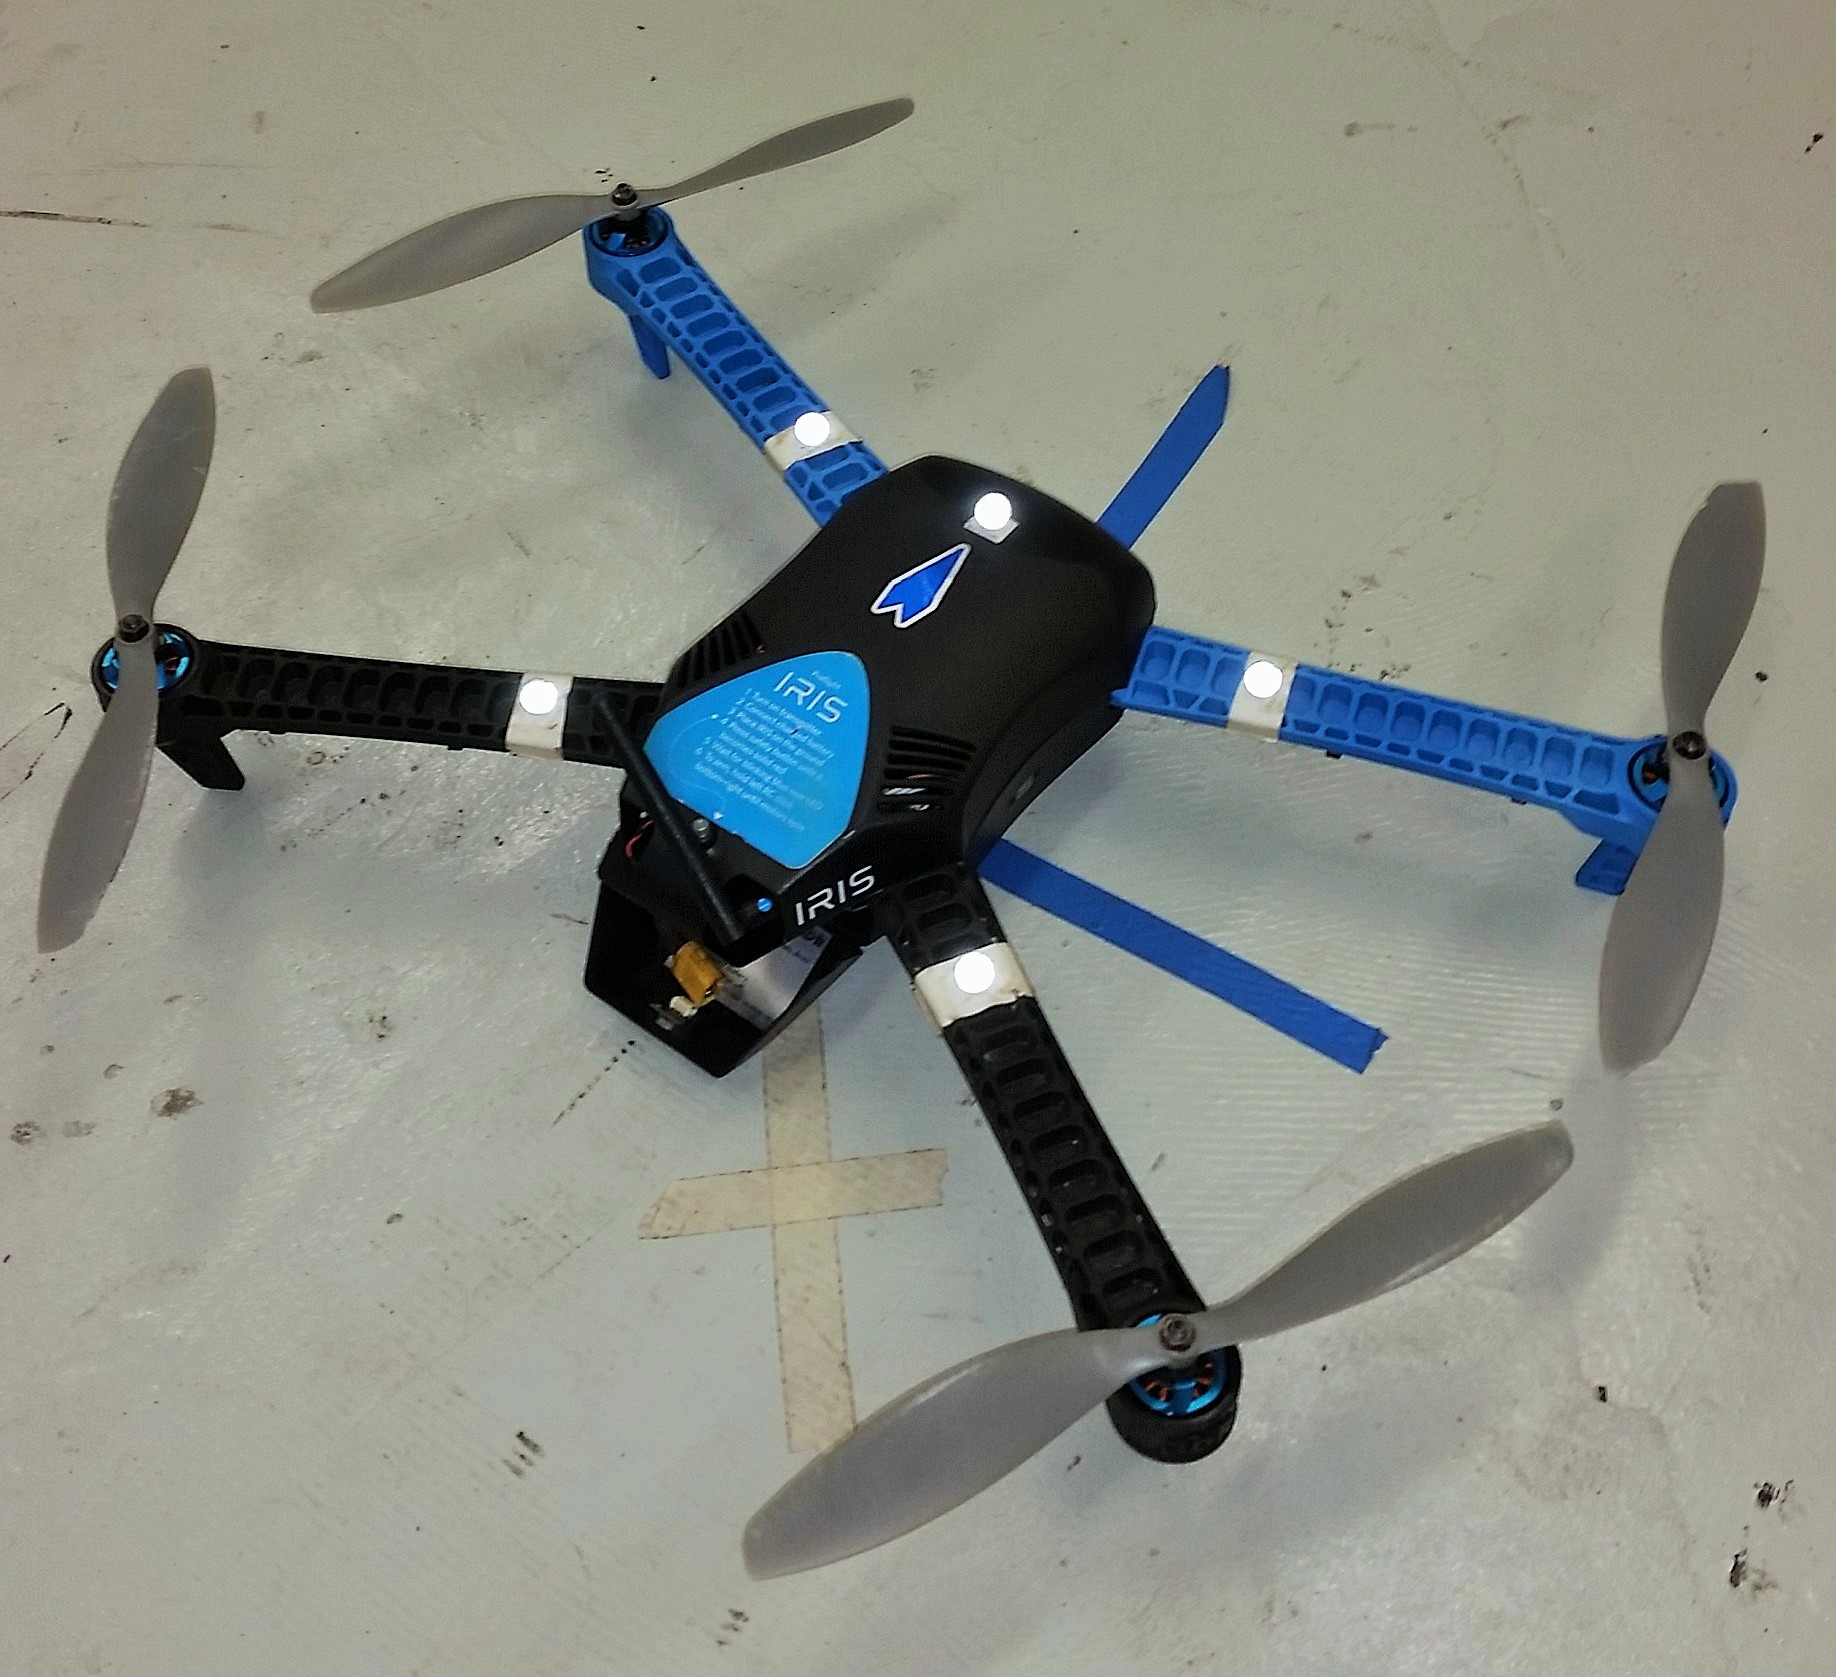
\includegraphics[width=0.6\textwidth]{irismarker.jpg}
 \caption[Marker placement on IRIS]{Markers placed on IRIS in asymmetrical 3D positions.}
 \label{figure:markedIRIS}
\end{figure}

\subsection{Flight Arena}
The flight arena is the stage of the setup. Since the laboratory where this thesis has taken place is new, I was involved in the relocation of the equipment from the old to the new lab. Next I attached every camera to the supports previously drilled on the roof and after I took care of the cables management. Since the maximum allowed length of the camera cables is 5 meters, I managed to place the hubs on the top at two opposite edges of the square (the ones intersecting x axis). By that, the available length is sufficient to connect three cameras of one edge and one from the adjacent edge to on hub and the rest to the other. The sync and the two hubs cables are running on the roof and crossing the room while the camera cables are displaced on the perimeter. Finally I oriented each camera towards the center of the room in order to have the highest coverage possible and calibrated the system.
\begin{figure}[h]
\centering
 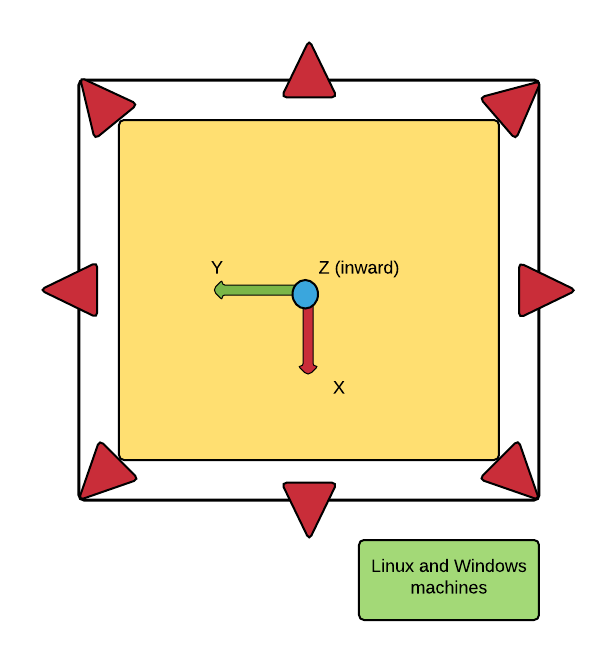
\includegraphics[width=0.6\textwidth]{flight_arena.png}
 \caption[Flight arena]{A scheme of the flight arena. In red there are the cameras, the yellow part is the flying space while the outer square is the protective net.}
 \label{figure:arena}
\end{figure}
\noindent
The flying space measures approximately 3 x 3 meters and 2 meters high defined by the capture volume of the mocap. Outside there is a security perimeter enclosing cameras made by a nylon net of about 4 x 4 meters till the roof. The origin of the position measures is at the center of the room placed on the floor with the z axis going downwards as shown in figure \ref{figure:arena}. A panoramic view of the arena, taken from the top left corner, is shown in figure \ref{figure:arenapano}. 

\begin{figure}[h]
\centering
 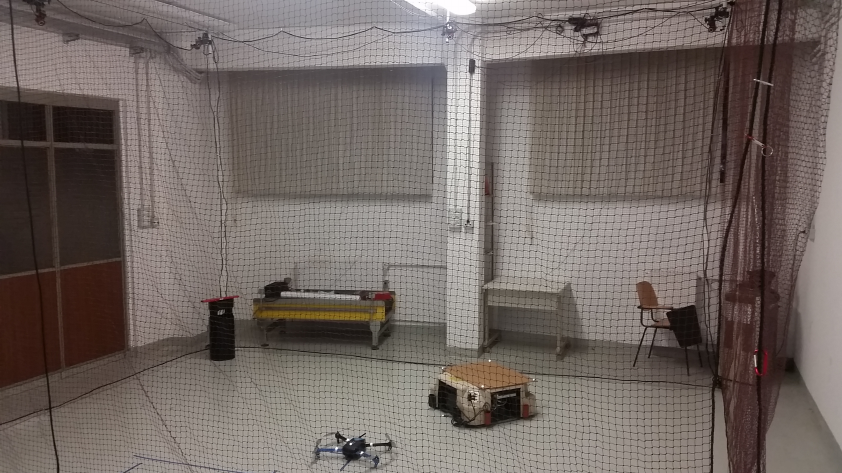
\includegraphics[width=0.8\textwidth]{panoramic.png}
 \caption[Flight arena panoramic]{Panoramic view of the flying space.}
 \label{figure:arenapano}
\end{figure}

\begin{figure}[h]
	\centering
	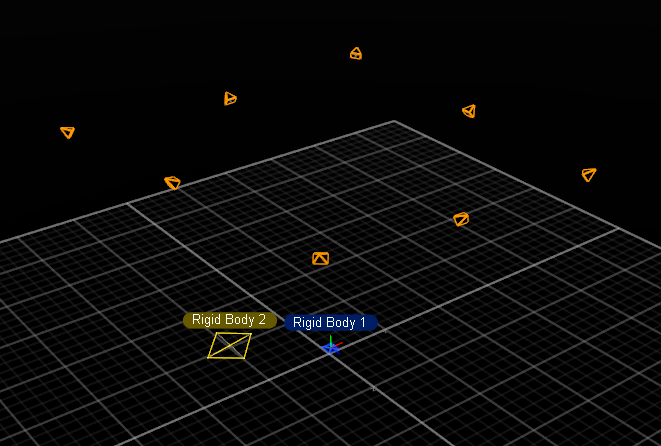
\includegraphics[width=0.6\textwidth]{motiv_panorama.PNG}
	\caption[Flight arena from motive]{Flight arena seen by Motive with a couple of rigid bodies and cameras.}
	\label{figure:arenamotive}
\end{figure}



\section{Overall Integration}
\label{sec:integration}

This section explains to the reader how every part of the setup is interfacing with each other, the flow of data packets from OptiTrack to IRIS and the operation done to the information at each step.

\subsection{Hardware interfaces}

Each camera is equipped with a 5 meters USB cable and, as stated in \ref{sec:mocap}, four cables are connected to one hub and four to the second hub. As outputs, the hubs are equipped with a 5 meter USB cable that can be expanded to 10 meters, those two connection are inputs for the Windows machine. \\*

\noindent
\textbf{Windows machine specs} 
\begin{itemize}

\item OS: Windows 7 
\item Processor: Intel i7 3.60 GHz
\item RAM: 32 Gb
\item Video Card: NVIDIA GTX 970
\item Software tools: Motive

\end{itemize}
This computer is directly connected to a Linux machine through Ethernet cable (RJ-45 connectors). \\

\noindent
\textbf{Linux machine specs} 
\begin{itemize}

\item OS: Ubuntu 14.04 LTS 
\item Processor: Intel i7 2.40 GHz
\item RAM: 8Gb
\item Video Card: NVIDIA GeForce GTX 760M
\item Software tools: Qt C++ Libraries, Px4 build environment \cite{PX4Build}
\end{itemize}
At the end, via USB , a telemetry module (Fig. \ref{figure:telemetry}) is attached to the linux machine.
\begin{figure}[h]
\centering
 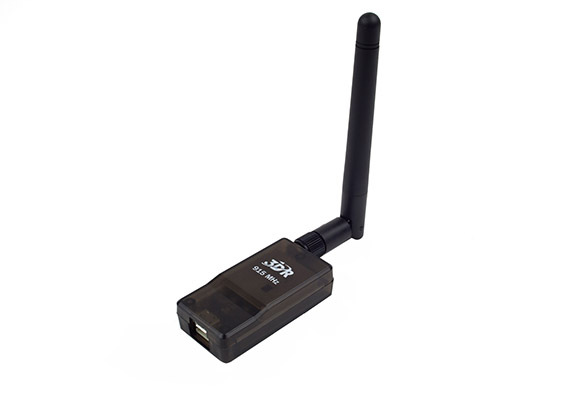
\includegraphics[width=0.6\textwidth]{telemetry.jpg}
 \caption[Telemetry module]{Telemetry module from 3d Robotics used to recieve and transmit MAVLink Packages with IRIS.}
 \label{figure:telemetry}
\end{figure}
This radio link allows the control station to communicate with the robot wirelessly with acceptable performance. It is mainly used for acquiring telemetry and robot status, transmit new mission goals, check robot parameters such as controller gains and calibrate onboard sensors. \\*

\noindent
Its main features are \cite{3Dr}:

\begin{itemize}
\item 433 MHz (for Europe).
\item micro USB port: it can be used also from tablets.
\item UART Interface.
\item 2-way full-duplex communication.
\item MAVLink protocol framing.
\end{itemize}
Moreover, IRIS features a standard RC transmitter, shown in figure \ref{figure:iris_planner}, from which the user can operate the robot in three main modes:
\begin{enumerate}
\item Fully manual: radio sticks control directly velocity of the propellers.
\item Semi-auto: height is stabilized, left stick control height position set point while attitude is manual.
\item Fully-auto: horizontal position is stabilized through position feedback, right stick controls x and y set points.
\end{enumerate}

\subsection{Software interfaces}

Motive has the feature to transmit the pose of every tracked rigid bodies through a multicast IP. By this option, the raw pose of the robot is transmitted to the Linux machine. The software architecture running on Linux reads data coming directly from Motive through a \textit{Receiver component}. Without the use of an \textit{adapter component}, since the program is specific for this application, data from Motive is processed as explained in section \ref{sec:adaptframes} at the moment it arrives. In the mean while a position set point is generated inside the architecture, both pose estimation and position set point are packed using MavLink protocol. At the end data is sent through a socket interface an the telemetry module takes care of transmitting everything to IRIS with a rate of approximately 10Hz.

Figure \ref{figure:integration} sums up in a scheme the relation between each part. 

\begin{figure}[h]
\centering
 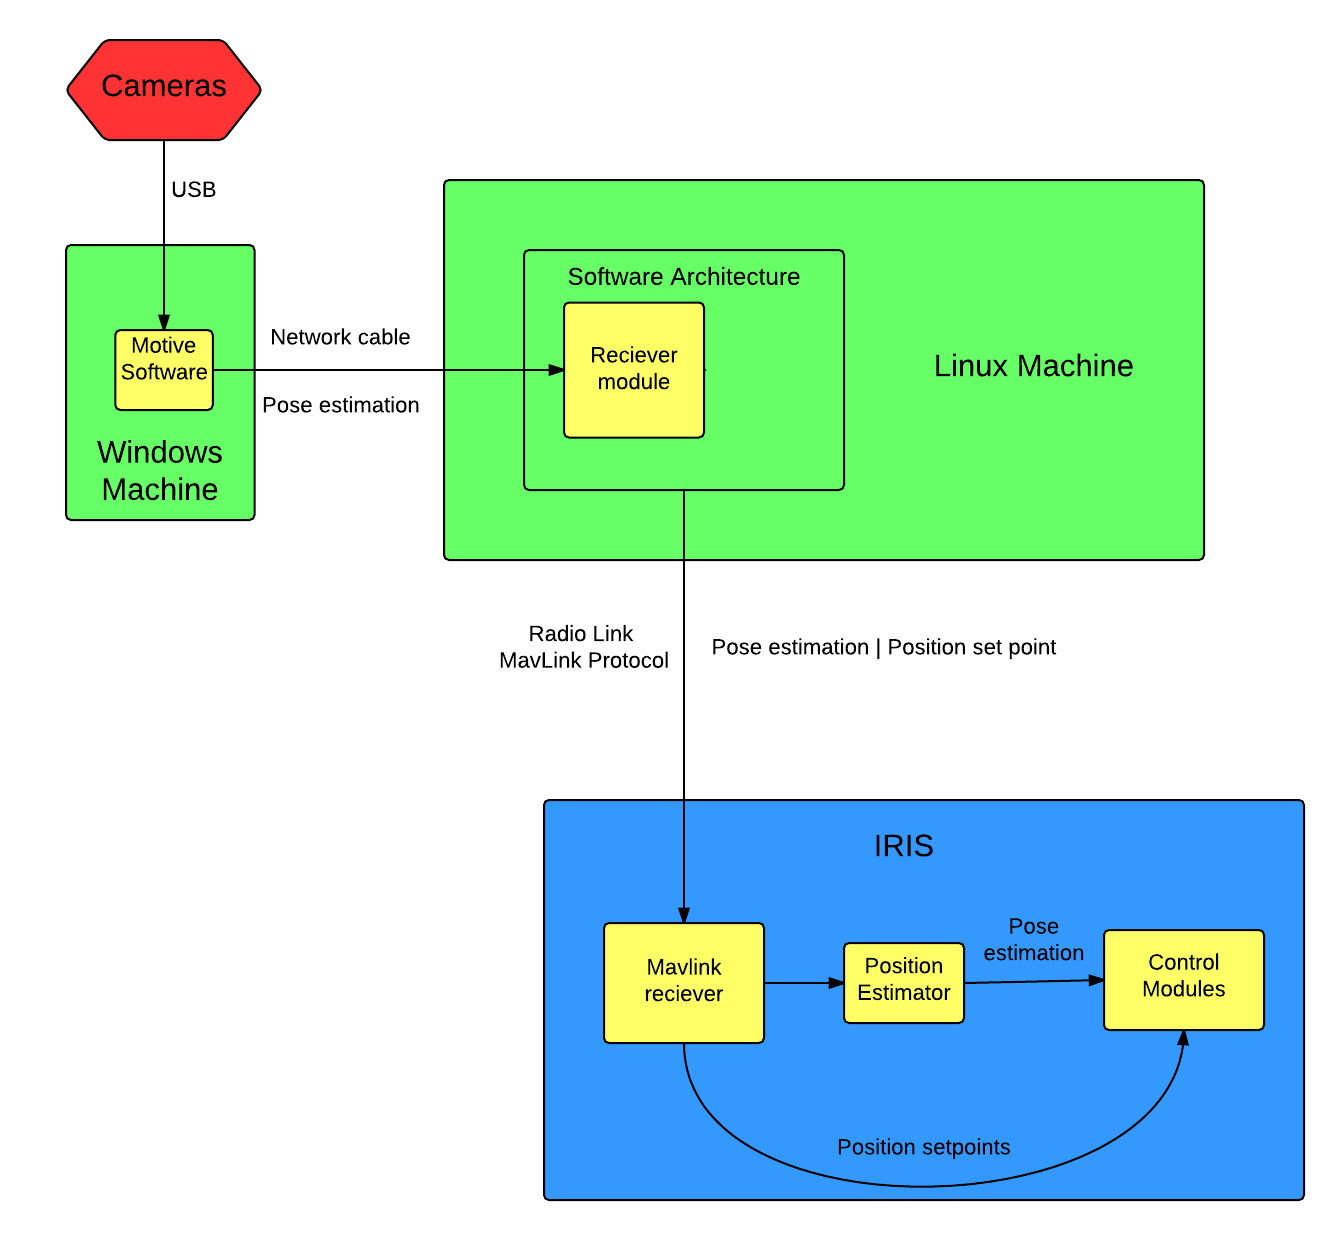
\includegraphics[width=0.9\textwidth]{integration.png}
 \caption[Setup scheme]{Scheme of the setup with connections between parts}
 \label{figure:integration}
\end{figure}

\subsubsection{Adapting reference frames}
\label{sec:adaptframes}
Motive transmits a 6 degree of freedom pose (position and orientation)respect to a fixed reference frame $\Re^m$ in the form:\\ 
\begin{equation}
Pose^m = \begin{bmatrix}
P^m\\
Q^m
\end{bmatrix}
\end{equation}
 where $P^m\ = \begin{bmatrix}x&&y&&z\end{bmatrix}^T$ is the position vector and $Q^m =\begin{bmatrix}w&&x&&y&&z\end{bmatrix}^T$ is the rotation quaternion, everything expressed in Motive reference frame $\Re^m$. \\
 
 \noindent
Now let us define a second reference frame, in this case is a North-East-Down frame \cite{FrameRef}  mainly used in aeronautics and aerial robotics, namely  $\Re^E$. The peculiarity of this reference is that:

\begin{itemize}
\item x axis is aligned with North.
\item y axis is aligned with East.
\item z axis goes down towards the earth.
\end{itemize}

\noindent
The only constraint of $\Re\textsuperscript{m}$ is that y is vertical and x parallel to the ground, hence x and y can be set freely at the moment of cameras calibration Figure \ref{figure:frames} shows both reference.

\begin{figure}[h]
\centering
 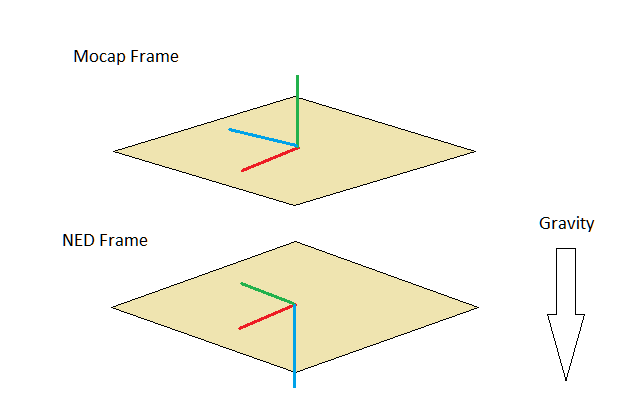
\includegraphics[width=0.8\textwidth]{frames.png}
 \caption[NED and Mocap frames]{NED and Mocap frames depicted. X axis in red, y axis in green and z axis in blue}
 \label{figure:frames}
\end{figure}

It is easily shown that the relation between frames is a 90 degree rotation of $\Re\textsuperscript{m}$ over x. Let $R_x(\theta)$ be the rotation matrix on x, $P^b$ arbitrary  3-elements vector column respect to a general base frame $b$, then the following is valid:
\begin{equation}
(P\textsuperscript{m})\textsuperscript{T}R_x(\theta) = P\textsuperscript{E}
\label{eq:adaptframe}
\end{equation}

\begin{equation}
R_x(\theta) = \begin{bmatrix} 1 & 0            & 0 \\
							  0 & \cos(\theta) & -\sin(\theta)\\
                              0 & \sin(\theta) &  \cos(\theta) 
\end{bmatrix}
\label{eq:rotx}
\end{equation}

By putting $\theta = \pi/2$ inside \eqref{eq:rotx}, \eqref{eq:adaptframe} becomes:

\begin{equation}
\begin{bmatrix}x&y&z\end{bmatrix}\begin{bmatrix} 1 & 0 & 0 \\
							  					 0 & 0 & -1\\
                              					 0 & 1 & 0
\end{bmatrix} = \begin{bmatrix}x\\z\\-y\end{bmatrix}
\label{eq:rotexplained}
\end{equation}

and

\begin{equation}
P\textsuperscript{E} = \begin{bmatrix}x\\z\\-y\end{bmatrix}
\label{eq:translation}
\end{equation}

where $[x, y, z]$ are the coordinates of $P^m$ in $\Re^m$.\\

\noindent
As regards the rotational part, some comments must be done. Since the applied rotation applied does not influence the estimated attitude, we can safely state that:

\begin{equation}
Q\textsuperscript{E} = \begin{bmatrix}
w\\x\\z\\-y
\end{bmatrix}
\label{eq:quaternion}
\end{equation}
where $[w, x, y, z]$ are the elements of $Q^m$.\\

\noindent
Equations \eqref{eq:translation} and \eqref{eq:quaternion} describe the relation between $\Re^m$ and  $\Re^E$ in a simple but effective way in fact just by changing the order of the elements of the pose coming out Motive, a pose that IRIS can understand is generated. 
    